

\tikzset{every picture/.style={line width=0.75pt}} %set default line width to 0.75pt        

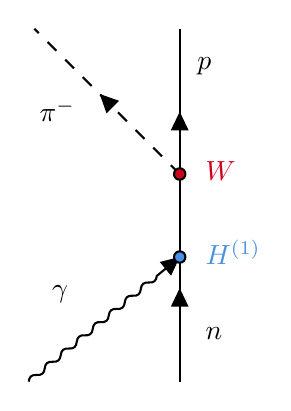
\begin{tikzpicture}[x=0.75pt,y=0.75pt,yscale=-1,xscale=1]
	%uncomment if require: \path (0,300); %set diagram left start at 0, and has height of 300
	
	%Straight Lines [id:da33488681649693186] 
	\draw    (270,210) -- (270,130) ;
	\draw [shift={(270,165)}, rotate = 90] [fill={rgb, 255:red, 0; green, 0; blue, 0 }  ][line width=0.08]  [draw opacity=0] (8.93,-4.29) -- (0,0) -- (8.93,4.29) -- cycle    ;
	%Straight Lines [id:da46389908648611555] 
	\draw    (197.25,210) .. controls (197.48,207.65) and (198.76,206.59) .. (201.11,206.82) .. controls (203.46,207.05) and (204.74,205.99) .. (204.96,203.64) .. controls (205.19,201.29) and (206.47,200.23) .. (208.82,200.46) .. controls (211.17,200.68) and (212.45,199.62) .. (212.68,197.27) .. controls (212.91,194.92) and (214.19,193.86) .. (216.54,194.09) .. controls (218.89,194.32) and (220.17,193.26) .. (220.39,190.91) .. controls (220.62,188.56) and (221.9,187.5) .. (224.25,187.73) .. controls (226.6,187.96) and (227.88,186.9) .. (228.11,184.55) .. controls (228.34,182.2) and (229.62,181.14) .. (231.97,181.37) .. controls (234.32,181.6) and (235.6,180.54) .. (235.82,178.19) .. controls (236.05,175.84) and (237.33,174.78) .. (239.68,175.01) .. controls (242.03,175.23) and (243.31,174.17) .. (243.54,171.82) .. controls (243.77,169.47) and (245.05,168.41) .. (247.4,168.64) .. controls (249.75,168.87) and (251.03,167.81) .. (251.25,165.46) .. controls (251.48,163.11) and (252.76,162.05) .. (255.11,162.28) .. controls (257.46,162.51) and (258.74,161.45) .. (258.97,159.1) -- (261.51,157) -- (267.69,151.91) ;
	\draw [shift={(270,150)}, rotate = 140.49] [fill={rgb, 255:red, 0; green, 0; blue, 0 }  ][line width=0.08]  [draw opacity=0] (8.93,-4.29) -- (0,0) -- (8.93,4.29) -- cycle    ;
	%Straight Lines [id:da3810232285211974] 
	\draw  [dash pattern={on 4.5pt off 4.5pt}]  (270,110) -- (200,40) ;
	\draw [shift={(231.46,71.46)}, rotate = 45] [fill={rgb, 255:red, 0; green, 0; blue, 0 }  ][line width=0.08]  [draw opacity=0] (8.93,-4.29) -- (0,0) -- (8.93,4.29) -- cycle    ;
	%Straight Lines [id:da6452866026111611] 
	\draw    (270,130) -- (270,40) ;
	\draw [shift={(270,80)}, rotate = 90] [fill={rgb, 255:red, 0; green, 0; blue, 0 }  ][line width=0.08]  [draw opacity=0] (8.93,-4.29) -- (0,0) -- (8.93,4.29) -- cycle    ;
	%Shape: Circle [id:dp14659197000759305] 
	\draw  [fill={rgb, 255:red, 74; green, 144; blue, 226 }  ,fill opacity=1 ] (267.25,150) .. controls (267.25,148.48) and (268.48,147.25) .. (270,147.25) .. controls (271.52,147.25) and (272.75,148.48) .. (272.75,150) .. controls (272.75,151.52) and (271.52,152.75) .. (270,152.75) .. controls (268.48,152.75) and (267.25,151.52) .. (267.25,150) -- cycle ;
	%Shape: Circle [id:dp1667146356512621] 
	\draw  [fill={rgb, 255:red, 208; green, 2; blue, 27 }  ,fill opacity=1 ] (267.25,110) .. controls (267.25,108.48) and (268.48,107.25) .. (270,107.25) .. controls (271.52,107.25) and (272.75,108.48) .. (272.75,110) .. controls (272.75,111.52) and (271.52,112.75) .. (270,112.75) .. controls (268.48,112.75) and (267.25,111.52) .. (267.25,110) -- cycle ;
	
	% Text Node
	\draw (281,182.4) node [anchor=north west][inner sep=0.75pt]    {$n$};
	% Text Node
	\draw (277,52.4) node [anchor=north west][inner sep=0.75pt]    {$p$};
	% Text Node
	\draw (201,72.4) node [anchor=north west][inner sep=0.75pt]    {$\pi ^{-}$};
	% Text Node
	\draw (207,162.4) node [anchor=north west][inner sep=0.75pt]    {$\gamma $};
	% Text Node
	\draw (281,140.4) node [anchor=north west][inner sep=0.75pt]  [color={rgb, 255:red, 74; green, 144; blue, 226 }  ,opacity=1 ]  {$H^{( 1)}$};
	% Text Node
	\draw (281,102.4) node [anchor=north west][inner sep=0.75pt]  [color={rgb, 255:red, 208; green, 2; blue, 27 }  ,opacity=1 ]  {$W$};
	
	
\end{tikzpicture}